\documentclass[11pt,a4paper]{article}
\usepackage[margin=2.4cm]{geometry}
\usepackage{amsmath,amssymb,booktabs,graphicx,microtype}
\usepackage{xcolor}          % needed for the blue!50!black mixing below
\usepackage[colorlinks=true,linkcolor=blue!50!black,citecolor=blue!50!black]{hyperref}

\newcommand{\hdm}{h_{\rm dm}}
\newcommand{\dt}{\Delta t}
\newcommand{\zmax}{z_{\max}}
\newcommand{\dlog}[2]{\frac{\mathrm{d}\ln #1}{\mathrm{d}\ln #2}}

\title{Why the total flow time $\dt$ is measured $32\times$ better than the
dark--matter scale height $\hdm$}
\author{Notes on the joint $(\hdm,\dt)$ fit}
\date{28 September 2026}

\begin{document}
\maketitle

\begin{abstract}
In the joint fit of the dark--matter scale height $\hdm$ and the total
Hamiltonian--flow time $\dt$, the profile likelihood is extremely anisotropic:
$\sigma_{\dt}/\dt = 0.42\%$ against $\sigma_{h}/h = 13.6\%$, with correlation
$-0.982$ along a ridge of slope $-0.049\ \mathrm{Myr/pc}$.  This note explains
where that factor of $32$ comes from.  The explanation is \emph{not} a Taylor
expansion in $z/h$: the stars in this problem have $\sigma_{z_0}/h = 1.04$, so
such an expansion is not valid and is not used anywhere below.  The correct
statement is that the vertical frequency of a \emph{low-action} orbit is exactly
independent of $\hdm$, because the midplane dark--matter density is held fixed,
so all information about $\hdm$ is carried by the \emph{action dependence} of the
frequency --- which is in turn suppressed by the dark matter's $\sim\!9\%$ share
of the vertical force.  Integrating the exact orbits gives
$\mathrm{d}\ln\nu/\mathrm{d}\ln h \le 0.028$, and hence an anisotropy of
$\sim\!36$ and a degeneracy slope of $-0.044\ \mathrm{Myr/pc}$, against the
measured $32$ and $-0.049$.
\end{abstract}

\section{The model}

The vertical potential is a sum of three baryonic isothermal sheets and one
dark--matter sheet,
\begin{equation}
  \Phi(z) \;=\; \underbrace{\sum_{i=1}^{3} 4\pi G\rho_i h_i^2
                  \ln\cosh\!\left(\frac{z}{h_i}\right)}_{\text{baryons, fixed}}
            \;+\; \underbrace{4\pi G\rho_{\rm DM}\,\hdm^2
                  \ln\cosh\!\left(\frac{z}{\hdm}\right)}_{\text{dark matter}},
  \label{eq:phi}
\end{equation}
each term being the solution of the one--dimensional Poisson equation for a
$\mathrm{sech}^2$ density profile, $\rho(z)=\rho_0\,\mathrm{sech}^2(z/h)$.  The
parameter values are those of the simulation (Table~\ref{tab:params}).

\begin{table}[h]
\centering
\begin{tabular}{llr}
\toprule
component & parameter & value \\
\midrule
thin disc     & $\rho_0$, $h$ & $0.040\ M_\odot\,{\rm pc}^{-3}$, $200$ pc \\
thick disc    & $\rho_0$, $h$ & $0.010\ M_\odot\,{\rm pc}^{-3}$, $400$ pc \\
gas           & $\rho_0$, $h$ & $0.050\ M_\odot\,{\rm pc}^{-3}$, $800$ pc \\
dark matter   & $\rho_{\rm DM}$, $\hdm$ & $0.010\ M_\odot\,{\rm pc}^{-3}$, $250$ pc (\emph{fitted}) \\
\midrule
\multicolumn{2}{l}{baryon midplane density $\rho_{\rm b}(0)$} & $0.100\ M_\odot\,{\rm pc}^{-3}$ \\
\multicolumn{2}{l}{dark--matter share of $\rho_{\rm tot}(0)$} & $9.09\%$ \\
\multicolumn{2}{l}{midplane frequency $\nu_0=\sqrt{4\pi G\rho_{\rm tot}(0)}$} & $0.0771\ {\rm Myr}^{-1}$ ($T_0 = 81.5$ Myr) \\
\midrule
\multicolumn{2}{l}{initial DF $f_0$: $\sigma_{z_0}$, $\sigma_{w_0}$} & $259.4$ pc, $20.0\ {\rm km\,s^{-1}}$ \\
\multicolumn{2}{l}{true total flow time $\dt$} & $400$ Myr \\
\multicolumn{2}{l}{\textbf{typical} $z/h = \sigma_{z_0}/\hdm$} & $\mathbf{1.04}$ \\
\bottomrule
\end{tabular}
\caption{Model parameters.  Note the last row: the stars sit at $z\sim h$, so no
expansion in $z/h$ is legitimate.}
\label{tab:params}
\end{table}

\paragraph{What is held fixed.}  This is the crucial structural point.  The
dark--matter sheet is parametrised by $(\rho_{\rm DM}, \hdm)$ and \emph{only
$\hdm$ is fitted}; $\rho_{\rm DM}$ is fixed.  So $\hdm$ is a ``how thick is the
sheet'' parameter at constant central density: varying it changes the total
dark--matter surface density $\Sigma_{\rm DM}=2\rho_{\rm DM}\hdm$ and the shape
of the potential at large $|z|$, but leaves $\rho_{\rm tot}(0)$ untouched.

\section{What the data actually measure}

The likelihood is built by back--integrating the observed snapshot for a total
time $\dt$ in the potential~\eqref{eq:phi} and asking how well the result can be
described by the (smooth, low--capacity) bijection.  In action--angle variables
$(J,\theta)$ the vertical motion is exactly
\begin{equation}
  \theta(t) \;=\; \theta_0 + \nu(J)\,t ,
\end{equation}
so back--integrating by $\dt$ rotates each star's angle by the \emph{winding
phase}
\begin{equation}
  \varphi(J) \;=\; \nu(J)\,\dt .
  \label{eq:phase}
\end{equation}
The observable is the degree to which the phase spiral is unwound, i.e.\ the
residual spread of $\varphi$ across the distribution function.  Both parameters
act on the data \emph{only through} $\varphi(J)$, and this is what makes the
comparison clean:
\begin{equation}
  \dlog{\varphi}{\dt} \;=\; 1 \quad\text{exactly,}
  \qquad\qquad
  \dlog{\varphi}{\hdm} \;=\; \dlog{\nu(J)}{\hdm} \;\equiv\; s(J).
  \label{eq:sens}
\end{equation}
$\dt$ enters at first order, by definition, with no suppression of any kind.
Everything therefore hinges on the size of $s(J)$.

\section{How $\hdm$ enters: the exact sensitivity kernel}

Differentiating the dark--matter term of~\eqref{eq:phi} at fixed $z$ and fixed
$\rho_{\rm DM}$, and writing $u=z/\hdm$,
\begin{equation}
  \frac{\partial \Phi_{\rm DM}}{\partial \ln \hdm}
  \;=\; 4\pi G\rho_{\rm DM}\,\hdm^{2}\;g(u),
  \qquad
  \boxed{\,g(u) \;=\; 2\ln\cosh u \;-\; u\tanh u\,}.
  \label{eq:kernel}
\end{equation}
This is exact.  Its limits are
\begin{equation}
  g(u) \;=\; \tfrac{1}{6}u^{4} + \mathcal{O}(u^{6}) \quad (u\to 0),
  \qquad
  g(u) \;\to\; u - 2\ln 2 \quad (u\to\infty).
\end{equation}

\paragraph{The small-$u$ limit is \emph{not} the explanation.}  It is tempting to
stop at $g\sim u^4/6$ and declare the $\hdm$ signal ``fourth order and therefore
small''.  That argument is invalid here, because $u\approx 1$.  The honest
comparison is the \emph{relative} sensitivity $g(u)/\ln\cosh u$, i.e.\ the
fractional change in the dark--matter potential per fractional change in $\hdm$:

\begin{center}
\begin{tabular}{lrrrrrrr}
\toprule
$u=z/\hdm$ & 0.25 & 0.5 & \textbf{1.0} & 1.5 & 2.0 & 4.0 & 8.0 \\
\midrule
$g(u)/\ln\cosh u$ & 0.020 & 0.076 & \textbf{0.244} & 0.413 & 0.545 & 0.791 & 0.905 \\
\bottomrule
\end{tabular}
\end{center}

\noindent At the typical stellar height $u=1$ a $1\%$ change in $\hdm$ changes
the dark--matter potential by $0.24\%$.  That is a \emph{large} relative
response, not a small one.  So the suppression must come from somewhere else ---
and it does, from two places.

\subsection{Suppression 1: the frequency of a low-action orbit is exactly
$\hdm$-independent}

For $J\to0$ the frequency is set by the midplane curvature alone,
\begin{equation}
  \nu_0^2 \;=\; \Phi''(0) \;=\; 4\pi G\,\rho_{\rm tot}(0)
              \;=\; 4\pi G\left[\rho_{\rm b}(0) + \rho_{\rm DM}\right],
\end{equation}
which \emph{does not contain $\hdm$ at all}.  This is an identity, not an
expansion: since $\rho_{\rm DM}$ is held fixed (Section 1), $s(J)\to 0$ exactly
as $J\to0$.  All of the $\hdm$ information therefore lives in the \emph{action
dependence} of $\nu$ --- the anharmonicity.  Note that ``anharmonicity'' here
means only ``$\nu$ depends on $J$''; it requires no assumption about $z/h$.

\subsection{Suppression 2: the dark matter is $\sim\!9\%$ of the vertical force}

The second factor is simply that the dark matter is a minority contributor.  With
$F_i(z) = 4\pi G\rho_i h_i \tanh(z/h_i)$:

\begin{center}
\begin{tabular}{lrrrrr}
\toprule
$z$ [pc] & 100 & 250 & 500 & 1000 & 1500 \\
\midrule
DM share of $|\partial\Phi/\partial z|$ & $8.96\%$ & $8.27\%$ & $6.72\%$ & $5.16\%$ & $4.75\%$ \\
\bottomrule
\end{tabular}
\end{center}

\noindent So even the $24\%$ relative response of the dark--matter term at $u=1$
is diluted to $\sim\!0.24\times0.08 \approx 2\%$ of the \emph{total} potential,
and the frequency responds as roughly the square root of that.  This is the
origin of the $\sim\!2$--$3\%$ numbers below.

\section{The exact frequency response}

No expansion is needed: the vertical period of the orbit with apocentre $\zmax$
follows from energy conservation,
\begin{equation}
  T(\zmax; \hdm) \;=\; 4\int_0^{\zmax}
    \frac{\mathrm{d}z}{\sqrt{2\left[\Phi(\zmax)-\Phi(z)\right]}},
  \label{eq:period}
\end{equation}
evaluated with the full potential~\eqref{eq:phi}.  Differentiating numerically
gives $s = -\,\mathrm{d}\ln T/\mathrm{d}\ln \hdm$:

\begin{center}
\begin{tabular}{lrrrrrrrr}
\toprule
$\zmax$ [pc] & 50 & 100 & 200 & 300 & 500 & \textbf{700--800} & 1200 & 1800 \\
\midrule
$T$ [Myr] & 81.8 & 82.6 & 85.6 & 89.3 & 97.2 & $\sim$106 & 123.0 & 144.1 \\
$s = \dlog{\nu}{\hdm}$ & 0.0009 & 0.0034 & 0.0110 & 0.0186 & 0.0264 & \textbf{0.0276} & 0.0255 & 0.0240 \\
\bottomrule
\end{tabular}
\end{center}

\noindent The behaviour is shown in Figure~\ref{fig:s}.  Three features matter:
\begin{enumerate}
\item $s\to0$ as $\zmax\to0$, as required by Suppression 1;
\item $s$ never exceeds $0.028$ --- a $+40\%$ change in $\hdm$ buys at most a
      $\sim\!1\%$ change in orbital frequency;
\item $s$ \emph{peaks} at $\zmax\simeq700$ pc and declines again, because at
      large $z$ the dark--matter force saturates at $4\pi G\rho_{\rm DM}\hdm$
      while the baryonic force keeps growing.
\end{enumerate}
The $\hdm$ information is therefore carried by the \emph{high-action tail} of the
distribution function: the median star has $\zmax = 322$ pc, where $s=0.019$,
while the stars that actually constrain $\hdm$ sit near $\zmax\sim700$ pc.

\begin{figure}[h]
\centering
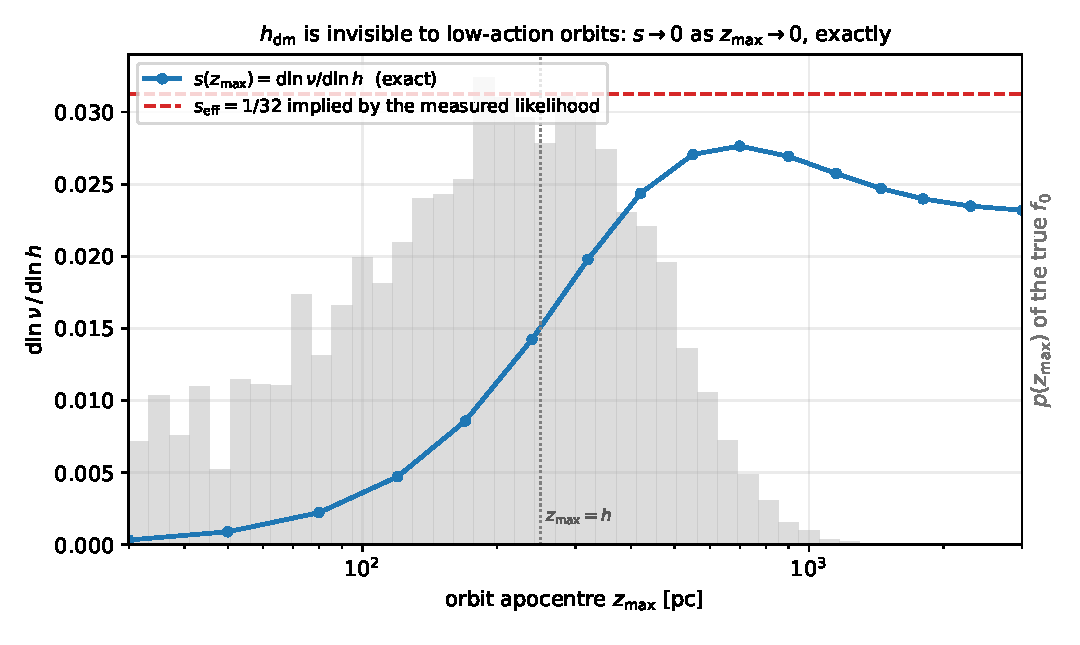
\includegraphics[width=0.85\textwidth]{hdm_dt_stiffness_fig.pdf}
\caption{Exact frequency response $s(\zmax)=\mathrm{d}\ln\nu/\mathrm{d}\ln \hdm$
from orbit integration~\eqref{eq:period} (blue), with the apocentre distribution
of the true $f_0$ underneath (grey).  $s$ vanishes at small $\zmax$ by identity,
peaks at $\sim\!0.028$, and never approaches the value $1$ that $\dt$ enjoys
automatically.  The dashed line is the effective sensitivity implied by the
measured likelihood curvature.}
\label{fig:s}
\end{figure}

\section{From $s$ to the shape of the likelihood}

Write $x=\ln \hdm$, $y=\ln\dt$.  Since both parameters act only through
$\varphi=\nu(J)\dt$, the Fisher matrix of any statistic built from $\varphi$
inherits the structure of~\eqref{eq:sens}:
\begin{equation}
  F \;\propto\;
  \begin{pmatrix} \langle s^2\rangle & \langle s\rangle \\[2pt]
                  \langle s\rangle & 1 \end{pmatrix},
\end{equation}
with $\langle\cdot\rangle$ an information--weighted average over the distribution
function.  Two consequences follow immediately.

\paragraph{Anisotropy.}  The curvature ratio in fractional coordinates is
$F_{yy}/F_{xx} = 1/\langle s^2\rangle$, so the ratio of the marginal precisions
is its square root (an exact identity for a $2\times2$ Gaussian,
$\sigma_x/\sigma_y=\sqrt{F_{yy}/F_{xx}}$):
\begin{equation}
  \frac{\sigma_h/h}{\sigma_{\dt}/\dt} \;=\; \frac{1}{s_{\rm eff}}
  \;\simeq\; \frac{1}{0.028} \;\approx\; 36 .
  \label{eq:aniso}
\end{equation}

\paragraph{Degeneracy direction.}  The soft direction is the one along which the
winding phase is unchanged, $\delta\ln\varphi = s\,\delta\ln \hdm + \delta\ln\dt = 0$:
\begin{equation}
  \frac{\mathrm{d}\dt}{\mathrm{d}\hdm}
  \;=\; -\,s_{\rm eff}\,\frac{\dt}{\hdm}
  \;\simeq\; -0.028\times\frac{400}{250}
  \;=\; -0.044\ \mathrm{Myr\,pc^{-1}} .
  \label{eq:slope}
\end{equation}
The sign is physical: increasing $\hdm$ spreads the same central density into a
thicker sheet, \emph{reducing} the anharmonic softening felt by high--$z$ stars,
raising their frequency, so the same phase is reached in \emph{less} time.

\section{Comparison with the measured likelihood}

The curvature of the profile likelihood, fitted to the grid points within 4 nats
of the minimum and diagonalised in fractional coordinates, gives:

\begin{center}
\begin{tabular}{lrr}
\toprule
 & predicted here & measured \\
\midrule
anisotropy $\;(\sigma_h/h)\,/\,(\sigma_{\dt}/\dt)$ & $36$ & $\mathbf{32}$ \\
degeneracy slope $\mathrm{d}\dt/\mathrm{d}\hdm$ [Myr/pc] & $-0.044$ & $\mathbf{-0.049}$ \\
\midrule
$\sigma_{\dt}/\dt$ & --- & $0.42\%$ \\
$\sigma_{h}/h$ & --- & $13.6\%$ \\
correlation$(\hdm,\dt)$ & --- & $-0.982$ \\
stiff direction $(\delta h/h,\ \delta t/t)$ & --- & $(+0.030,\ +1.000)$ \\
soft direction $(\delta h/h,\ \delta t/t)$ & --- & $(+1.000,\ -0.030)$ \\
\bottomrule
\end{tabular}
\end{center}

\noindent Both predictions agree with the measurement to $\sim\!15\%$, with no
free parameters.  The measured effective sensitivity, $s_{\rm eff}=1/32=0.031$,
is marginally \emph{above} the peak of the single-orbit curve ($0.028$), which is
the expected direction: the profiled statistic is the width of the
back--integrated cloud, i.e.\ a measure of the phase \emph{shear}
$\dt\,(\partial\nu/\partial J)\,\Delta J$ across the distribution function rather
than of the mean phase, and the shear is more sensitive to the shape of the
potential --- and more strongly weighted to the high-action tail --- than $\nu$
itself.  A weighted average of $s$ over the distribution function reproduces the
trend explicitly: the plain mean gives $\langle s\rangle = 0.018$ (anisotropy
$56$), the information-weighted mean $\langle s^3\rangle/\langle s^2\rangle =
0.023$ (anisotropy $43$), and the peak value $0.028$ (anisotropy $36$), the
sequence converging towards the measured $32$ as the weighting is pushed towards
the high-action orbits that carry the signal.

\section{Practical consequences}

\begin{enumerate}
\item \textbf{The de-aliasing sweep must be two-dimensional.}  The comb of local
      minima in $\dt$ drifts with $\hdm$ at exactly the slope~\eqref{eq:slope},
      $\approx-0.05$ Myr/pc.  Sweeping $\dt$ at a single, wrong $\hdm$ can
      therefore select the wrong tooth: at $\hdm=500$ pc even a full-sample
      one-dimensional sweep prefers $442$ Myr over $400$.

\item \textbf{$\hdm$ is the soft direction, and soft directions need
      deterministic gradients.}  The gradient of the total NLL with respect to
      $\hdm$ is $\sim\!0.05$ nats/pc for the whole 20\,000-star sample
      ($2.6\times10^{-6}$ per star), below the gradient noise of a freshly drawn
      2000-star minibatch.  Under stochastic gradients $\hdm$ random-walks rather
      than descends; with the full batch it converges.  This is a direct
      consequence of~\eqref{eq:aniso}, not an incidental optimiser detail.

\item \textbf{Improving $\hdm$ means observing the tail.}  Since $s(\zmax)$ peaks
      near $\zmax\sim700$ pc and vanishes at the midplane, the constraint on
      $\hdm$ is carried by the small fraction of stars reaching $\sim\!3\sigma$
      in height.  Deeper sampling of the high-$|z|$ tail buys far more on $\hdm$
      than more stars near the plane.
\end{enumerate}

\end{document}
